\documentclass[msthesis.tex]{subfiles}

\begin{document}
\chapter{Results}
\label{chap:results}
In this section, the quantitative and visualization results from the methods presented in \autoref{chap:methods} will be presented. The first two sections will present results from preprocessing of the \gls{DWI} images mentioned in \autoref{sec:Diffusionimgprepro} and extraction of connectivity matrices. The subsequent sections will describe the nature of the acquired data as well as classification results based on the comprehensive classification parameters illustrated in \autoref{tab:classify_combo}.

\section{Preprocessing Visualization}
\begin{figure}
    \centering
    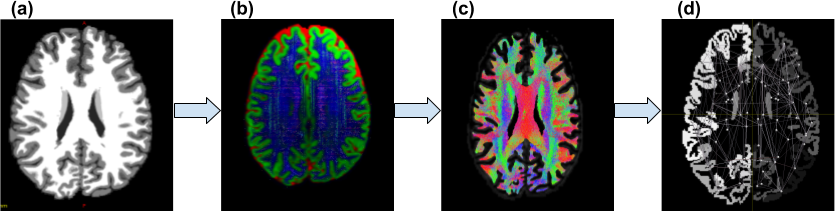
\includegraphics[width=\textwidth]{images/Preprocessing_pipeline.png}
    %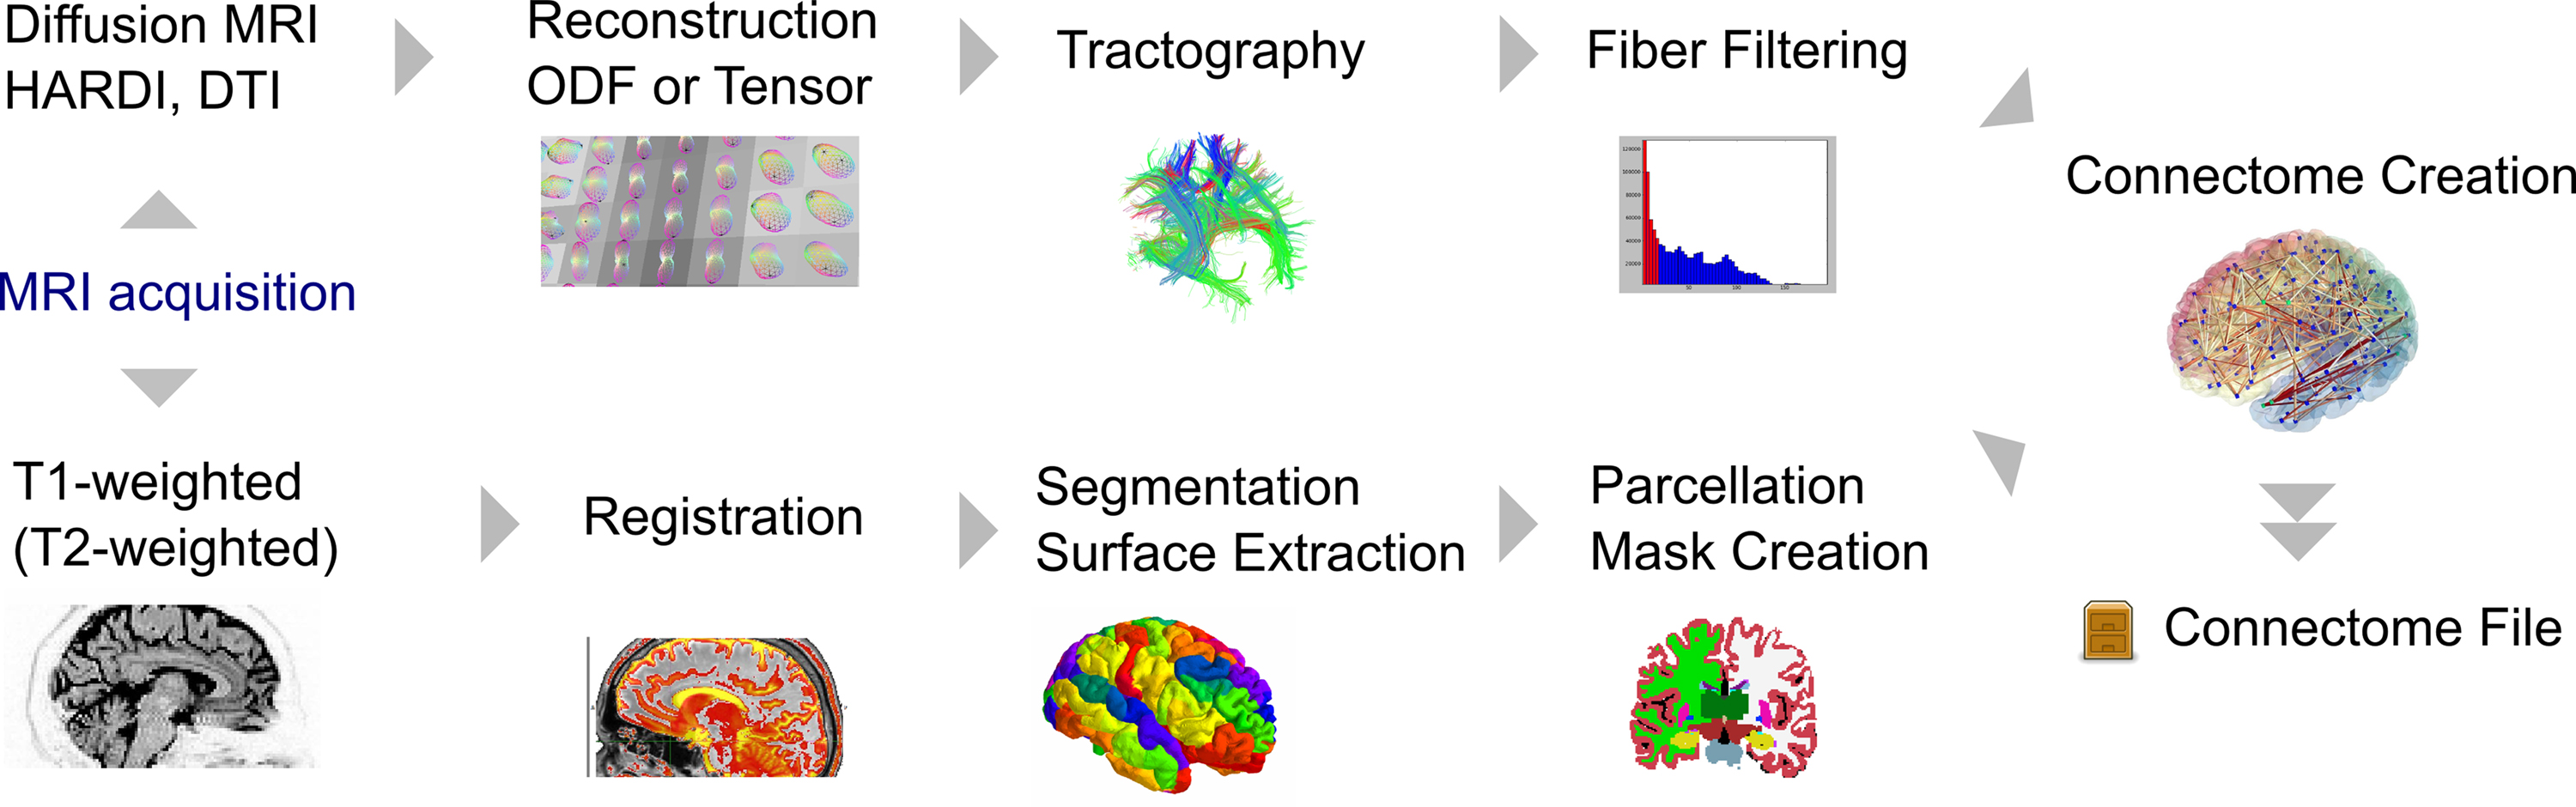
\includegraphics[width=\textwidth]{images/connectome_creation_workflow.png}
    %\cite{gerhard2011connectome}
    \caption{Visualization of pipeline used to create a connectome for each subject on an axial slice (a) Five tissue segmented image visualized in grayscale. (b) A slice of a 4D image mapped in 3D using RGB encoding tissue densities, CSF as red, GM as green and WM as blue. (c) \gls{ACT} of one million fibers overlaid on an axial slice of the brain. (d) Visualization of the spatial location of the center of masses of different \gls{ROI}s.}
    \label{fig:preproc}
\end{figure}

During the process of generating the connectome (\autoref{subsec:connectomegeneration}) visual inspection was required to investigate the properties of different types of images produced. The results illustrated in \cref{fig:preproc} were used to evaluate the adherence of the implementation to the conceptual framework mentioned \autoref{sec:creating_connectome}. 

The \gls{5TT} image obtained after tissue segmentation (\autoref{subsec:struct_diff}) was 4D and could not be easily displayed in 3D. In \cref{fig:preproc}.a this 4D image is displayed according to gray-scale mapping in 3D. The intensity of the background was set to 0,  that of cortical gray matter at 0.5, subcortical gray matter at 0.75, white matter at 1, CSF at 0.15 and pathological tissue at 2. With this gray-scale mapping, it was visually observed that the \gls{5TT} images did not contain any erroneous labels.

\iffalse
    -bg value image intensity of background (default: 0)
    -cgm value image intensity of cortical gray matter (default: 0.5)
    -sgm value image intensity of sub-cortical gray matter (default: 0.75)
    -wm value image intensity of white matter (default: 1)
    -csf value image intensity of CSF (default: 0.15)
    -path value image intensity of pathological tissue (default: 2)
The original 4D image contained three volumes with each one representing the corresponding tissue densities of \gls{WM}, \gls{GM} and \gls{CSF} image with each volume getting its specific color, i.e. \gls{WM} as blue, \gls{GM} as green and \gls{CSF} as red. In an interactive window from \textbf{\textit{mrview}} \citep{tournier2019mrtrix3} the \gls{RGB} image can be zoomed in to check for anatomical correspondence of the tissue densities. 
\fi
Three different volumes containing the tissue densities of \gls{WM}, \gls{GM} and \gls{CSF} are obtained by determining the corresponding \gls{fODF}s using \gls{MSMT-CSD}. The three images were then concatenated to a 4D image with \gls{RGB} encoding: \gls{CSF} as red, \gls{GM} as green and \gls{WM} as blue.  In \cref{fig:preproc}.b, the 4D image is visualized as an \gls{RGB}. Using an interactive window from \textbf{\textit{mrview}} \citep{tournier2019mrtrix3} the \gls{RGB} image was zoomed and checked for compliance of the response functions with the \gls{fODF}s and tissue segmentations.

After obtaining information about the tissue segmentations and \gls{fODF}s, one million fibers whole brain tractography was generated (\cref{fig:preproc}.c). In this tractogram the red fibers run in the right to left direction, green ones in anterior-posterior and blue in head-to-foot direction \citep{hobert2013evaluation}. Finally, the connectome was visualized (\cref{fig:preproc}.d) with the nodes representing the center of mass of different gray matter regions and the edges as the connections between them. The intensity of this image is not equal to the signal intensity but the number assigned to the ROI, so any \gls{ROI} that has a higher numbering in the lookup table is shown brighter (see Appendix). 

Overall, visualizing the preprocessing pipeline helped to evaluate the anatomical correspondence of the tractography. It also helps understand the relationship between the generated connectome and white matter structural brain connectivity.

\section{Connectome Visualization}

\begin{figure}
    \centering
    %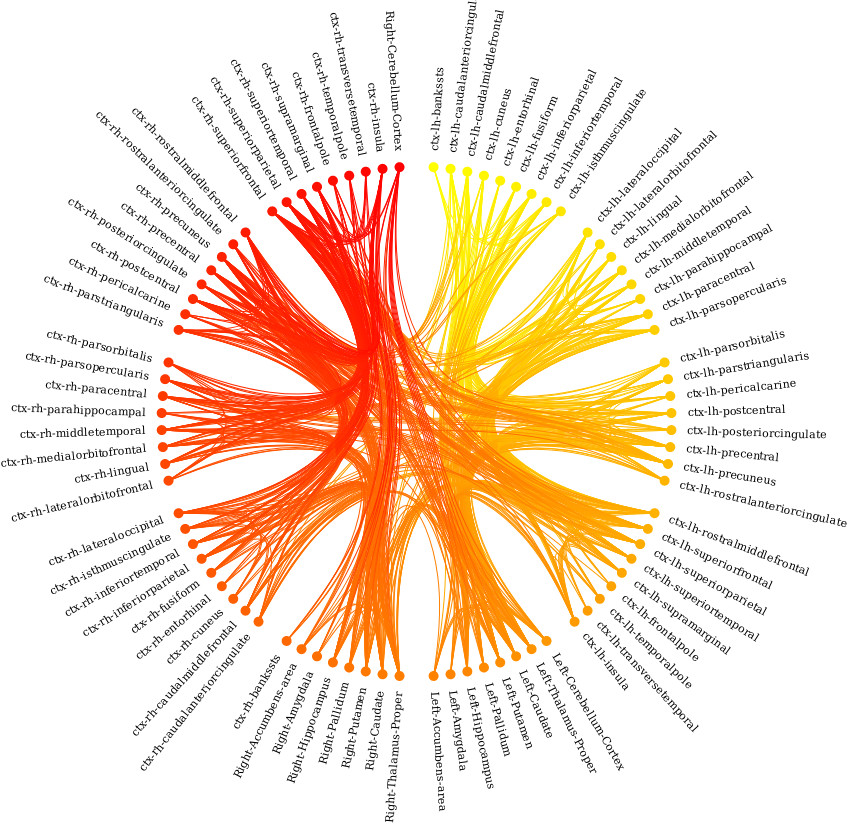
\includegraphics[width=\textwidth]{images/brain-data-viewer_2.png}
    %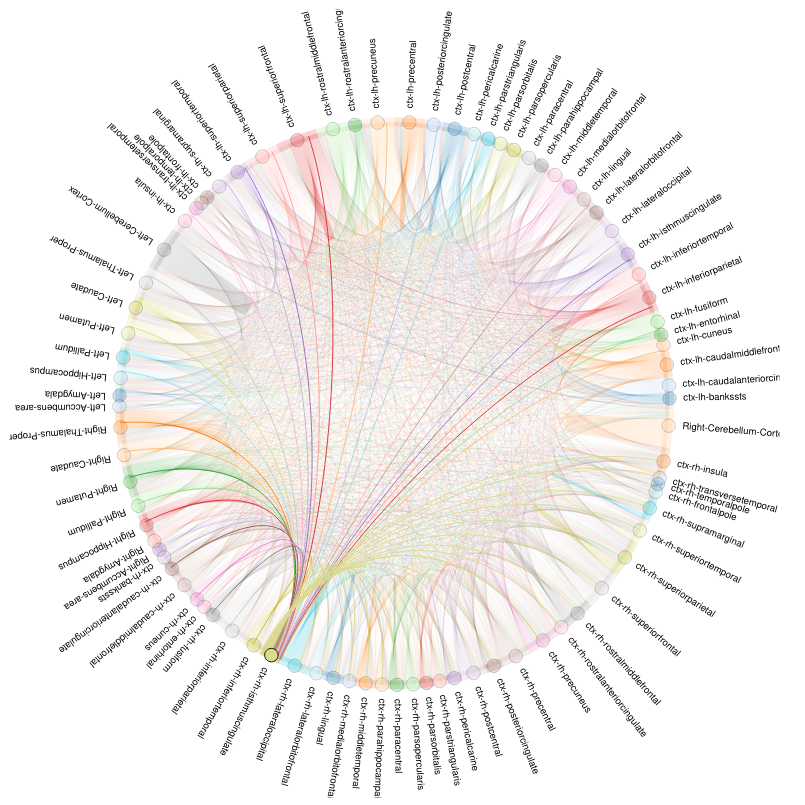
\includegraphics[width=\textwidth]{images/bokeh_plot_allsubjects.png}
    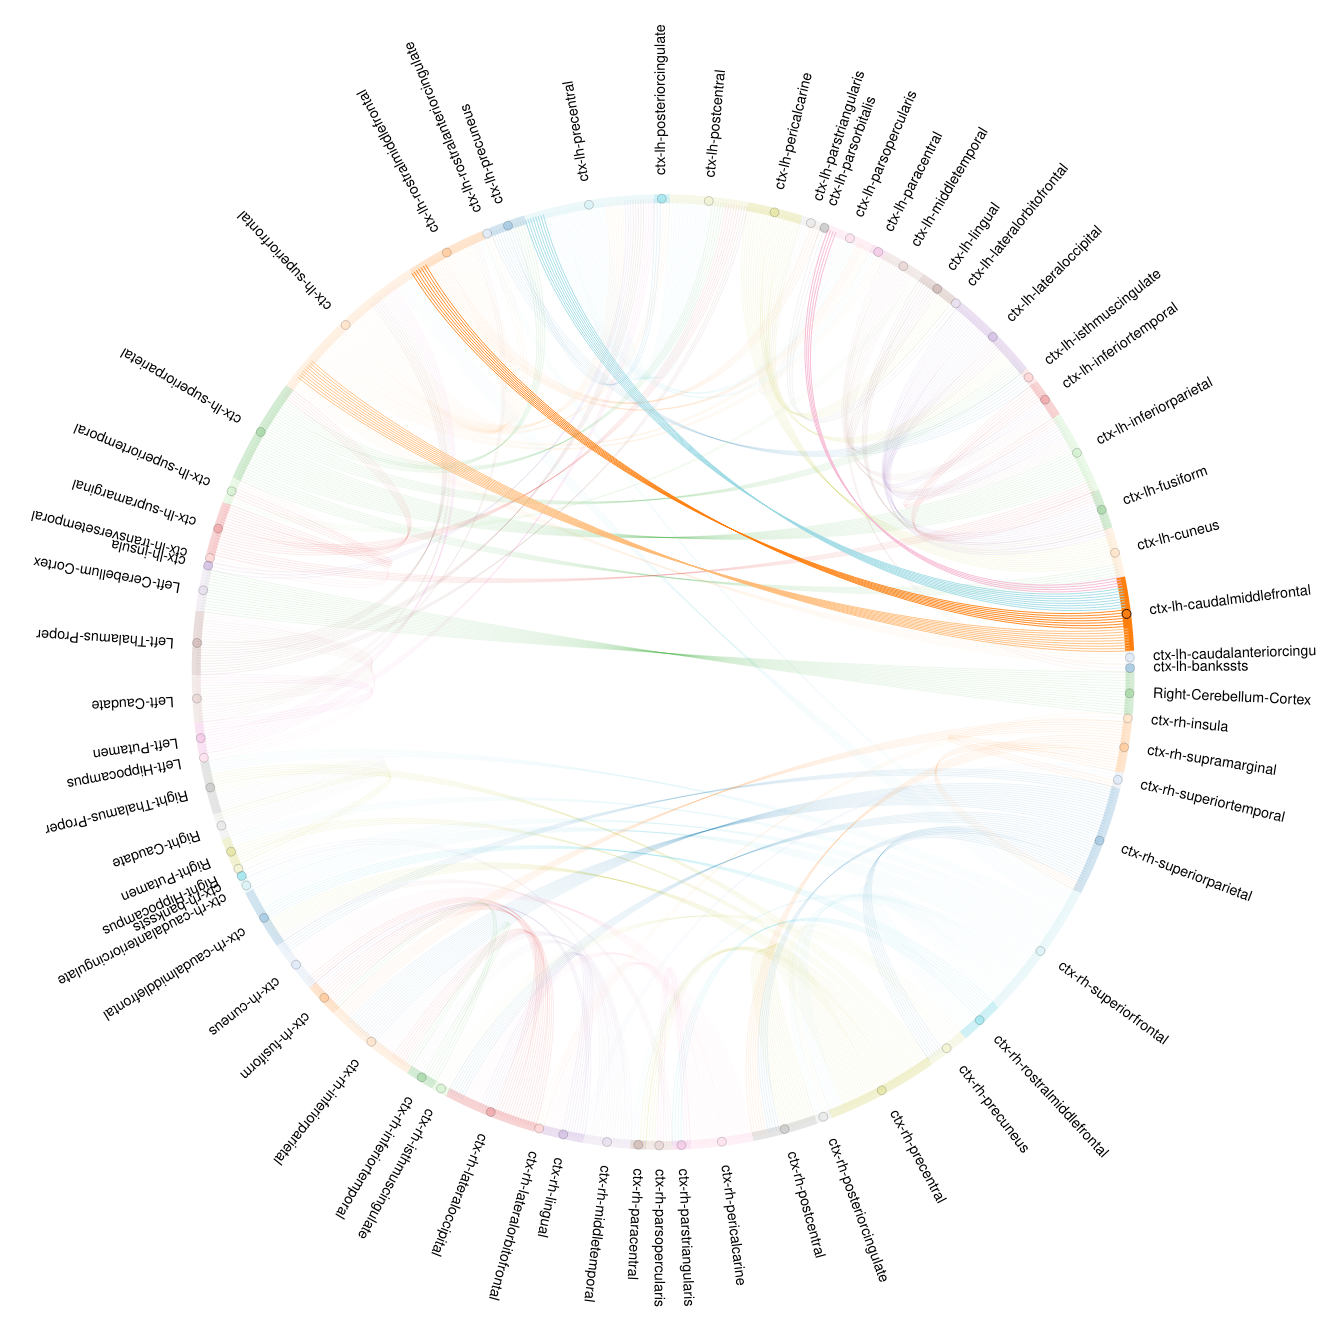
\includegraphics[width=\textwidth]{images/selected_view_all.png}
    \caption{A chord plot representing the group averaged connectome for all subjects. Nodes at the end of the circle correspond to \gls{ROI}s. The thickness of each edge corresponds to the number of arcs between two \gls{ROI}s. The number of arcs is proportional to the number of streamlines. In this interactive visualization the selected node (middle frontal gyrus in the left hemisphere) and its corresponding edges are highlighted while the other proprieties are made transparent. Edges connecting the selected node and target nodes are colored according to the target nodes. For example, the arcs are blue colored when there are connections to the precuneus in the left hemisphere.}
    \label{fig:connectome_num_streamlines}
\end{figure}

After the connectivity matrices for all subjects were generated using the methods in \autoref{sec:creating_connectome}, a group averaged connectome was created. The raw connectivity matrix was dense, containing $n = 84$ nodes and $n_e = 3486$ edges. The edge weights were widely distributed for all the three connectivity metrics: mean FA, mean streamline length, and number of streamlines. Visualizing the connectome as a simple connectivity matrix or a heatmap was hence not an effective strategy.

A chord plot was chosen to represent structural brain connectivity because of the ease of representing gray matter nodes along the boundary of the graph. It is an effective way of visualizing the flow between different nodes. The number of streamlines could be easily encoded within a chord plot since the number of arcs drawn between any two nodes can be specified. The reason for the selection of the number of streamlines as a connectivity metric for structural brain connectivity representation will be presented in \autoref{subsec:connmetric}.

The \cref{fig:connectome_num_streamlines} has been created with help of package \textit{holoviews} \citep{stevens2015holoviews}. In this figure, average number of streamlines (for all subjects) between any two regions are visualized, $n=65$ nodes are shown. Each node is assigned a different color according to the color palette in \textit{holoviews} \citep{stevens2015holoviews}. The arcs in the graph have been obtained by thresholding the group averaged number of streamlines between any two ROIs. This threshold was selected to be $N=900$. Only the connections which have more than $900$ streamlines are shown. The plot represents the number of streamlines along the preserved connections scaled down by a factor of $10$ for ease of representation.

The detailed coloring scheme used for creating the chord plot gives added visual cues about the source and the target nodes. Once a node is selected the edges get colored according to the color of the target node. As an example, the cortical region caudal middle frontal in the left hemisphere is selected in \cref{fig:connectome_num_streamlines}. It has prominent connections to the cortical regions superior frontal, rostra middle frontal and precuneus in the left hemisphere. A weak connection to the cortical region parsopercularis is also well represented by this diagram. 

Overall, this comprehensive diagram is a systematic representation of whole brain connectivity. It can be used to analyze brain connections at the subject level or the group level.

\section{Feature Analysis}
\label{features}
Once the connectivity matrices were ready, it was important to investigate an effective connectivity metric and determine importance of within \gls{ROI} connections. From the preprocessing pipeline presented in \autoref{subsec:connectomegeneration} there were three types of connectivity metrics obtained for each subject: number of streamlines, the mean streamline length and the mean FA. Each of these features encodes a different biological property of ROI-to-ROI connections and gave different classification results. There is no current consensus on which feature qualifies as an effective measure of connectivity between any two nodes \citep{yeh2020mapping}. The number of streamlines was selected to be the major focus of the classification tasks due its superiority in classification performance, which will be illustrated subsequently. Further, exclusion of self loops from the connectivity matrices will be experimentally justified. 

\subsection{Differences in Connectivity Metric}
\label{subsec:connmetric}
\begin{figure}
    \centering
    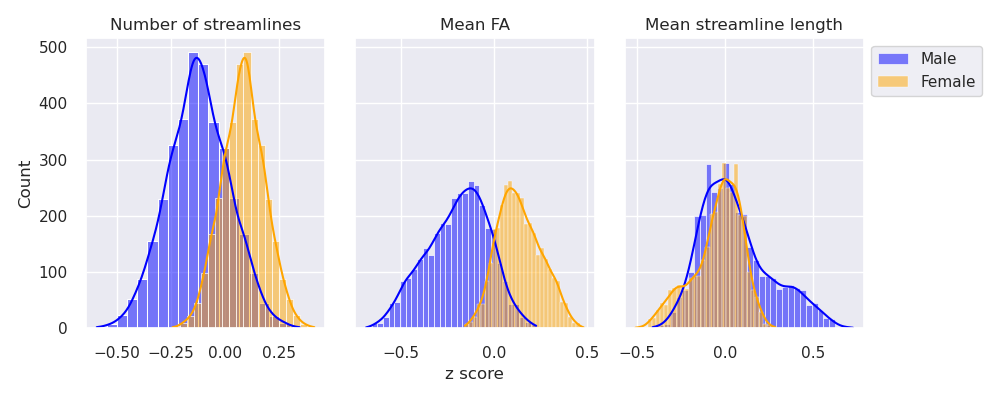
\includegraphics[width=\textwidth]{images/zscoredist.png}
    \caption{Three overlaid histograms representing the frequency of mean z-scores for different types of features. The orange histograms are for females and blue ones are for males. The y-axis represents the number of between ROI connections.}
    \label{fig:hist_zscores}
\end{figure} 
As mentioned above, it was important to explore different types of connectivity metrics obtained from the connectivity matrices constructed using the methodology illustrated in \cref{fig:connectivity_matrix}. Evaluation of z-score distributions of \gls{ROI} connections separately for males and females was taken as a method for data evaluation. Two overlaid histograms for each of the three different connectivity types helped speculate how well they separate between the two classes.

The histograms were formed using data (containing both data samples from males and females) in the training set. Each feature was standardized by removing the mean and scaling it to unit variance. After scaling the feature value for each subject could be represented by a z-statistic. As expected, the mean of the z-statistic (of one feature) was zero for all training subjects. However, the differences were prevalent when separate means were taken separately for the two genders. Hence, for each connection there was one z-score for males and another for females depending on the connectivity metric. For each connectivity metric, there are 3486 features considering pairwise connections excluding self loops (\autoref{sec:exclusion}) in an undirected graph. This number corresponds to the total count represented in \cref{fig:hist_zscores}.

From these distributions, it can be inferred that the number of streamlines have characteristics that can help interpret gender differences in structural brain connectivity. Its histograms show a smooth Gaussian distribution for males and females, and has significantly higher peaks than those for the other two features. Even though the mean FA features have a smaller overlap visually, the spread of its histograms is greater than that for the streamline count. The histograms of the mean streamline length are overlapping and skewed.

From the differences in z-score distribution, it can be inferred that women on an average have more number of streamlines as compared men in view of the same connections. This observation is coherent with evidence in \cite{szalkai2015graph} showing that women have more densely connected brains than men. Further, women have higher white matter to gray matter ratio and hence the number of streamlines detected for women is higher \citep{taki2011correlations}.

The mean \gls{FA} plots illustrate that women have higher mean FA values than men. An inconclusive trend is seen in the case of mean streamline length. Currently, there are no conclusive results for benchmarking such a distribution of \gls{FA} values, most results depend on the ROIs being considered \citep{kanaan2012gender}. It is difficult to conclude that female brains have higher FA values since existing studies in whole brain connectivity do not provide conclusive results \citep{ingalhalikar2014sex}. The mean streamline length remains a relatively unexplored connectivity metric hence substantial reasoning cannot be provided for explaining the trend of streamline lengths in \ref{fig:hist_zscores} \citep{BAJADA2019164}.  The difficulty of interpreting the mean \gls{FA} as well as mean streamline length is detailed in \autoref{disc:connfe}.

The results for the number of streamlines are coherent with \textit{a priori} knowledge and evidence in literature. The tractography was carried out in individual subject's space which could have caused biases in the comparison of fiber count between different subjects. Such biases were corrected for comparing the streamline count or length for different subjects using informed filtering from the \gls{SIFT} algorithm \citep{yeh2020mapping}. The \gls{SIFT} algorithm maps the reconstructed \gls{fODF}s back to the original \gls{dMRI} data. It then modifies the streamlines in accordance with image data and hence improves the biological correspondence of the streamline count. With this model, the number of streamlines becomes proportional to the total cross-sectional area of the white matter fibers connecting any two \gls{ROI}s. This proportionality makes the streamline count an interpretable connectivity metric as the the cross-sectional area of white matter pathways is of high anatomical correspondence \citep{SMITH2015253}. 

The experiments stated above and classification results in \autoref{subsec:Baseline_ana} help establish the advantage of streamline count as a connectivity metric as compared the other two metrics. It gives a biologically coherent measure of brain connectivity and achieves better performance than mean \gls{FA} and mean streamline length. 

\subsection{Self Loops}
\label{res:selfloops}

\begin{table}
\begin{tcolorbox}
\begin{tabular}{|p{0.135\textwidth}|l|l|l|l|}
\specialrule{0.2em}{0.01em}{0.01em}
\textbf{Label}& \textbf{ Metric}&\textbf{Feature}&\textbf{T statstic }&\textbf{P value}\\
\specialrule{0.2em}{0.1em}{0.1em}
Personality &Balanced&Mean FA&-0.196&0.846\\
Traits&accuracy&Mean streamline length&0.156&0.876\\
&&Number of streamlines &-1.248&0.217\\
&Area under &Mean FA&0.071&0.944\\
&ROC curve&Mean streamline length&1.332&0.188\\
&&Number of streamlines&-1.42&0.161\\
\specialrule{0.1em}{0.1em}{0.1em}
Gender&Balanced&Mean FA&0.396&0.695\\
&accuracy&Mean streamline length&2.068&0.048\\
&&Number of streamlines&0.98&0.335\\
&Area under &Mean FA&0.491&0.627\\
&ROC curve&Mean streamline length&3.875&0.001\\
&&Number of streamlines&2.199&0.036\\
\hline
\end{tabular}
\caption{Results for a paired samples t-test on the test set. The paired samples are the classification metrics of the data with and without the inclusion of self loops. The p values correspond to the t-test of two set of observations for the same classification metric constructed using methodology in \autoref{sec:exclusion}.}
\label{table:selfloops_combined}
\end{tcolorbox}
\end{table}

Evaluation of the importance of self loops was carried out on the basis of the experiment mentioned in \autoref{sec:exclusion}. The results in \autoref{table:selfloops_combined} were obtained by training the baseline experiments with and without the exclusion of self loops.  The report values correspond to classification performance on the test data. A positive t-statistic in this case indicates that the classification performance is greater with the inclusion of self loops. Meanwhile,  a negative t-statistic indicates the opposite trend. Statistical inference on this data indicates that the exclusion of self loops from the data analysis does not have a statistically significant effect on classification accuracy.  The statistics obtained from the analysis of both the target labels, i.e. the personality traits and gender labels do not lie in a significant confidence interval. The p-values in \autoref{table:selfloops_combined} are indicative of these results with most of them $p > 0.05$. 

Consider the statistics for the mean FA feature. All the p-values are $p>0.05$ and the t-statistic has opposite signs when it comes to considering two cases for personality classification. The first being balanced accuracy and the second as the \gls{AUC}. The t-statistic for the first case is $t=-0.196$ and for the second case is $t=0.071$. This opposite trend for two different  measures is indicative of the fact that there is no general trend of classification performance. 

With this investigation it became clear that the self loops can be eliminated from the data of all subjects. This ensured that the \gls{MEWIS} solver based technique as well as the baseline filters features from the same set of raw data.

\section{Baseline Analysis}
\label{res:baseline}

The baseline analysis mentioned in \autoref{subsec:Baseline_ana} with the parameter $k$ denoting the percentage of features to be preserved chosen to select the best performing connectivity metric. Initally, $k \in \{2,5,10,50,100\}$ was chosen to see an overall trend of classification performance. One important research question to be explored with this analysis was to determine whether doing any feature selection gives an added advantage for classification performance.

From  the results in \cref{fig:baselinegender}  it became evident that the number of streamlines served as a good metric for gender classification. There was only a loss of around 5\% performance for \gls{AUC} while reducing the percentage of features from 100\% to 5\% for both types of edge representations i.e. the t-test and f-scores and all three classifiers. In terms of number of features this meant that choosing just 175 out of 3486 features most of the discriminative information could be preserved.

Another consideration for gender classification was that even though the p-values of the t-test were scaled according to the function $f(x)= (-1) \times log_{10} p_{x}$ and the raw f-scores were used for scoring, the performance of the baseline analysis remained similar. In our training data the number of males and females were not equal and hence a Welsch's t-test assuming similar variances of the feature for the two groups was applied (\autoref{subsub:statcoef}). This could have introduced slightly different ranking from the f-scores as compared to the t-test.

\begin{figure}[]
    \centering
    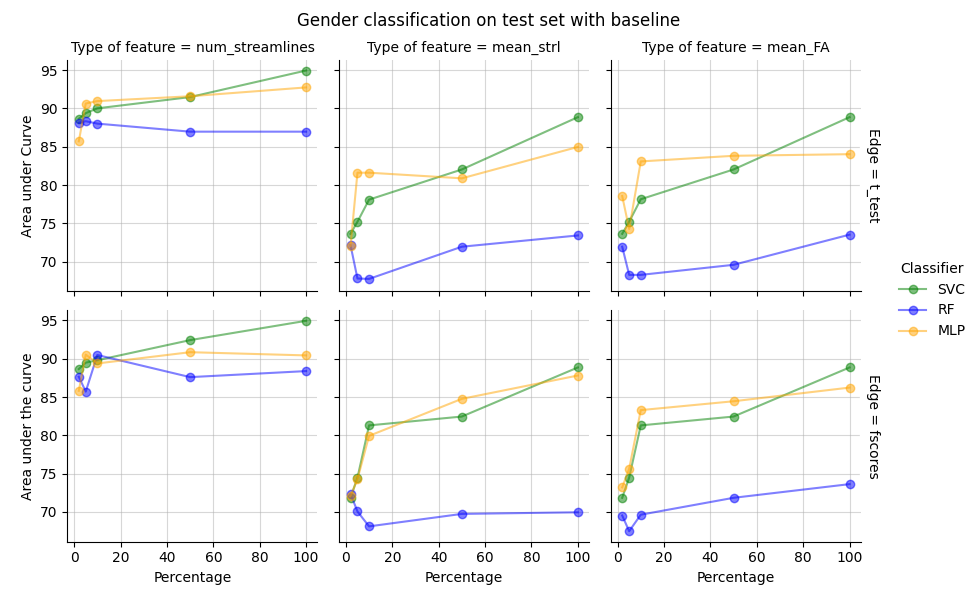
\includegraphics[width=\textwidth, height=0.6\textwidth]{images/baseline_results_gender.png}
    \caption{Baseline analysis for gender classification. The \gls{AUC} is represented as a function of percentage of features preserved. The three columns correspond to three different metrics used to represent structural brain connectivity. For the experiments illustrated in the first row the edges are filtered according to the p-value of the t-test and in the second row filtering is done using f-scores. }
    \label{fig:baselinegender}
\end{figure}
\begin{figure}[]
    \centering
    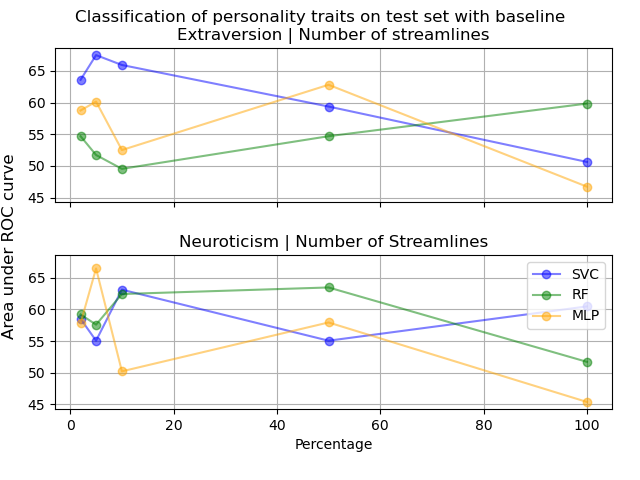
\includegraphics[height=0.4\textwidth,width=0.6\textwidth,keepaspectratio]{images/persona_2.png}
    \caption{Baseline analysis on the basis of personality traits using Pearson correlation coefficient as a filter method. For neuroticism, there is a trend of increase in performance with only a subset of original features using all three classifiers. For this particular configuration feature selection lead to much improved classifier performance with all three classifiers. A steep increase can be seen for extraversion where the \gls{AUC} increases from about 50\% (random chance) to about 68\%.}
    \label{fig:persona base}
\end{figure}

The classification of the different personality traits was more complex as compared to gender classification. All the possibilities of connectivity metrics and five different personality traits with Pearson correlation coefficient as the feature scoring were considered in the pipeline. However, an overall trend could be observed only with neuroticism and extraversion. For the traits openness and 
conscientiousness, the classification performance was often worse with feature selection than without. Hence, it could not be concluded that doing feature selection for personality traits is profitable. Only a subset of the experiments with the personality traits neuroticism and extraversion using streamline count as valid connectivity are mentioned according to \autoref{subsec:connmetric}. From the results in our analysis, it could be concluded that personality traits cannot be accurately classified using structural brain connectivity.

In \cref{fig:persona base} for neuroticism, there is a trend of increase in performance with only a subset of original features using all three classifiers. The trend for the \gls{MLP} shows greater than 65\% \gls{AUC} for top 5\% of features while 45\% without any feature selection. Classification performance on extraversion label increases with decrease in the number of features for classification with \gls{MLP} and \gls{SVC}. The strongest trend seen with the SVC, the \gls{AUC} increases from 50\% (without feature selection) to around 67\% (using top 5\% of the original features). The overall trend for neuroticism and extraversion illustrates that it is useful to do some feature selection in order to predict these traits

For gender classification, an interpretability-performance trade-off was observed. This trade-off is between the interpretability inversely proportional to the number of features and classifier performance that is directly proportional to the number of features. Feature selection seems profitable since the interpretability increases many fold when the number of features reduces from 3486 to just 175. 

The case for classification of personality traits is however different. Feature selection seems profitable in some cases but not all. In this section only the configurations for which feature selection shows an added advantage have been shown. For the selected configurations, classification based on the features selected by the \gls{MEWIS} solver features is significantly better than the non-informed baseline feature selection.

\section{Tracing Back to Original Features}
A major motivation behind implementing the \gls{MEWIS} based technique for this thesis was interpretability of the feature selection. In this section the interpretability of the set of features selected by the baseline as well as the solver based implementation are compared. It is observed that the solver based method is superior to the traditional baseline method due to connectedness of the output features. 

The two subsequent subsections present visualizations for the features selected by both the feature selection techniques. Furthermore, the \autoref{subsec:solverfeat} provides an insight into how the solver implementation preserves edges. 
\subsection{Subgraph Features}
\label{subsec:solverfeat}
For classification with the solver based technique detailed in \autoref{sec:MEWS}, the number of nodes preserved could be specified using a parameter $m$. Determining the order of growth in the number of edges as a function of $m$ was important to trace back the MEWIS selected features to the original \textit{dataframe}. \Cref{fig:fun_num_edges} shows a quadratic form with the number of edges $y$ as a function of the number of nodes $x$. This behavior is expected as the graph is supposed to be connected; i.e. there exists an edge between any two nodes in the graph. Using these results, the extent of interpretability from the solver results could be controlled. 
\begin{figure}
    \centering
    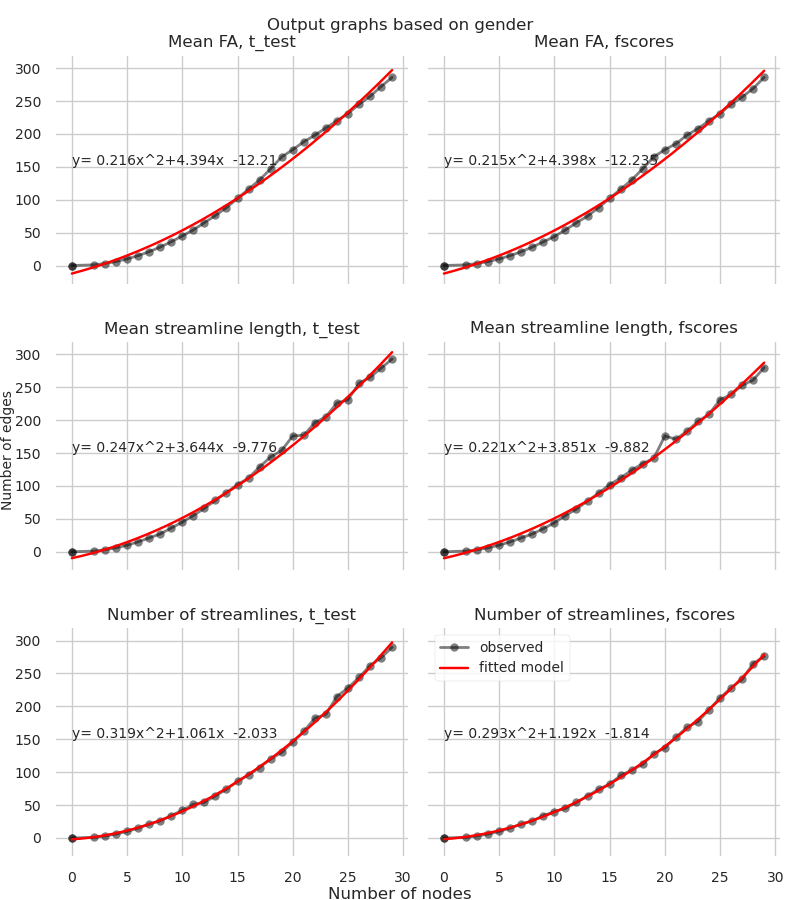
\includegraphics[height=0.5\textwidth,width=0.5\textwidth, keepaspectratio]{images/Gender_nodes_preserved.png}
    \caption{The number of edges preserved by the \gls{MEWIS} solver as a function of the number of nodes supplied to the  parameter $m$ (Eq. \ref{eq:sum_constraints}). The black dots illustrate the number of edges preserved for inputs  $m \in [4,30]$. A quadratic curve was fitted to map this trend. The red line represents the fitted model with the parameters mentioned in the figure. Using the fitted polynomial the number of edges preserved could be predicted before running the solver. This saved computational time and effort since the nature of output graphs could be predicted beforehand.}
    \label{fig:fun_num_edges}
\end{figure}

\subsection{Baseline-Solver Comparison}
\begin{figure}
    \centering
    %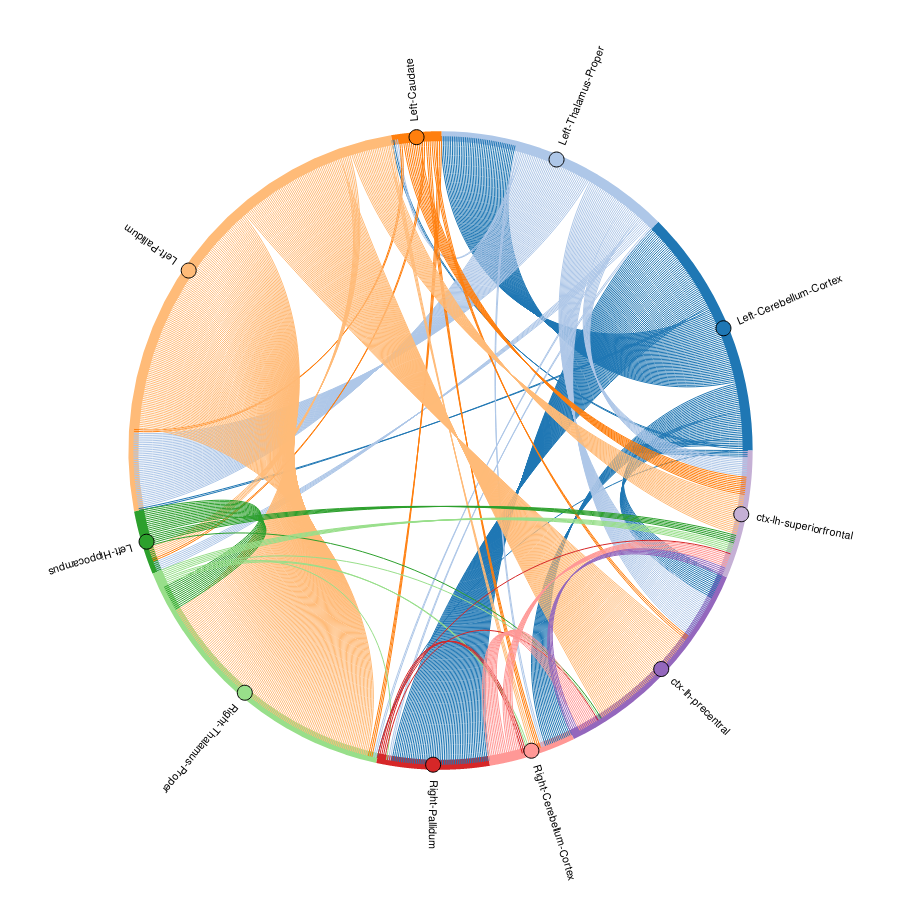
\includegraphics[width=0.9\textwidth]{images/gender10nodes_numstrls.png}
    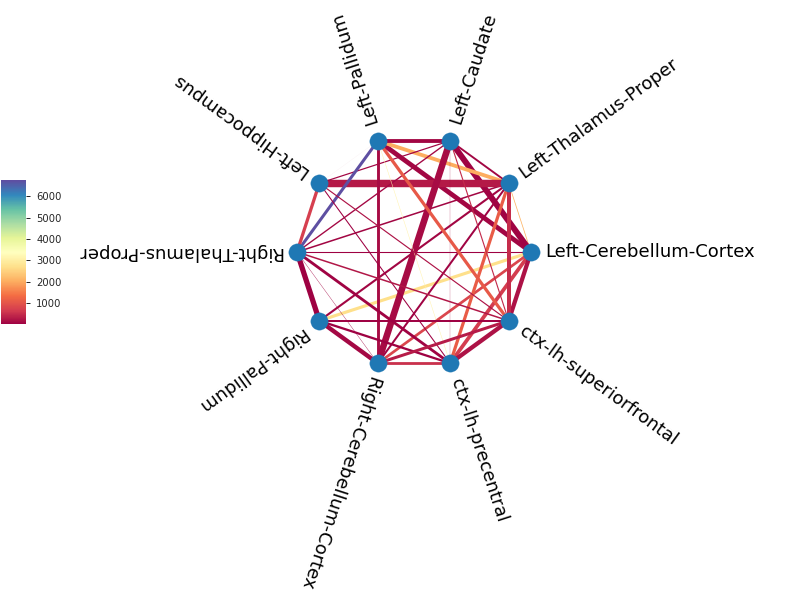
\includegraphics[width=\textwidth]{images/solver_10nodes_strls.png}
    \caption{10 most important nodes out of out of 84 determined using the \gls{MEWIS} solver for gender classification. The edge widths represent the f-scores of and color represents the number of streamlines between the two regions. A higher number of streamlines does not directly correspond to a higher f-score. 6 of the 10 selected nodes are subcortical regions; the thalai, the pallidai, the left hippocampus and left caudate while the remaining are cortical regions. This figure depicts that gender differences might be more prominent in subcortical brain networks than cortical brain networks. }
    \label{fig:gender_num_strls_10}
\end{figure}

\begin{figure}
    \centering
    %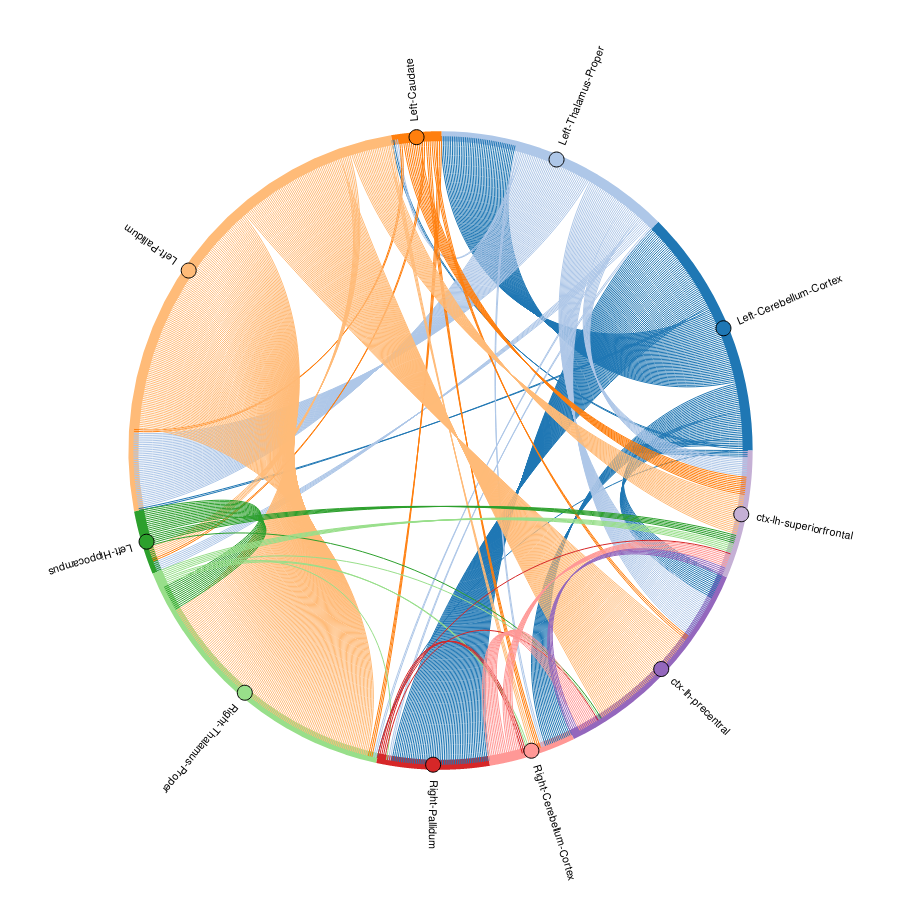
\includegraphics[width=0.9\textwidth]{images/gender10nodes_numstrls.png}
    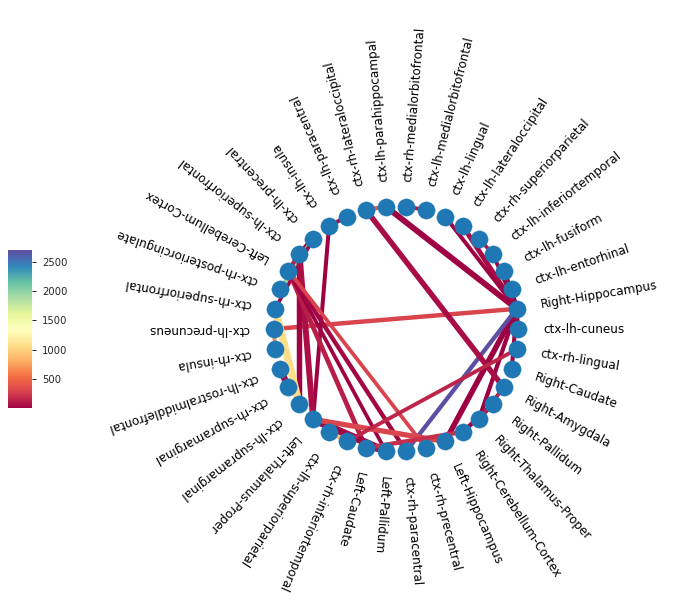
\includegraphics[width=0.7\textwidth]{images/baseline_42f_10nodes.png}
    \caption{41 most important features, and consequently 38 nodes preserved using baseline analysis for gender classification. The edge widths represent the f-scores and color represents the number of streamlines between the two regions. This figure shows that the baseline analysis does take graph topology into account and the features selected by this technique are not informative about any patterns such as the ones inferred using  MEWIS solver in \cref{fig:gender_num_strls_10}.}
    \label{fig:baseline_num_strls_10}
\end{figure}

In order to compare the two feature selection techniques, a separate input graph had to be created for a two use cases according to \autoref{tab:classify_combo}. These two use cases were visualized to compare the interpretability of predictions from the solver and baseline analysis.

In the first use case, the type of feature is number of streamlines, the target label is gender, edge representation is f-score and feature selection is solver with 10 nodes preserved in the subgraph. In the second use case, all the parameters were the same as the first use case except for baseline as the feature selection technique and number of edges as 41 for comparison with 41 edges preserved in the first use case (using polynomial in \cref{fig:fun_num_edges}).  The visualizations of these two use cases are \cref{fig:gender_num_strls_10} and \cref{fig:baseline_num_strls_10}. In both the visualizations, the edge widths represent the f-scores and the color represents the group averaged number of streamlines. The group averaged number of streamlines and f-scores are determined on the training data only. 

In \cref{fig:gender_num_strls_10} the MEWIS solver based implementation reduces the input graph and preserves 10 nodes along with 41 edges. It can be seen that the graph is well connected and structured. 6 out of 10 most important nodes are subcortical gray metter regions. These 6 regions are the thalai, the pallidai, the left hippocampus and left caudate. The lookup table from the Desikan-Killiany Atlas had total 68 nodes for cortical gray matter regions and 16 nodes for subcortical gray matter (see Appendix). The ratio of selected nodes for subcortical regions $0.375$ is higher than for cortical regions $0.058$. Such a pattern indicates that gender differences might be more prominent in networks of subcortical regions rather than cortical ones. \Cref{fig:baseline_num_strls_10} exemplifies the fact that the baseline method selects the same number of edges i.e. 41 as the solver by preserving 38 nodes, almost four times the nodes preserved by the solver. The graph is not connected and contains isolated edges, very often nodes with a degree of only 1 are seen.

\Cref{fig:gender_num_strls_10} and \cref{fig:baseline_num_strls_10} illustrate the superiority of the MEWIS solver generated subgraphs over baseline features in terms of interpretability. In a research setting, the MEWIS solver method would be more beneficial since it provides more interpretable results. With this technique it becomes easier to determine the subnetworks related to a particular target variable. 


\section{Model Performance}

Classification performance on the target label varied depending on the parameters of the data given to the classifier according to \autoref{tab:classify_combo}. This section will present the classification results for solver and personality traits respectively.
\begin{figure}[]
    \centering
    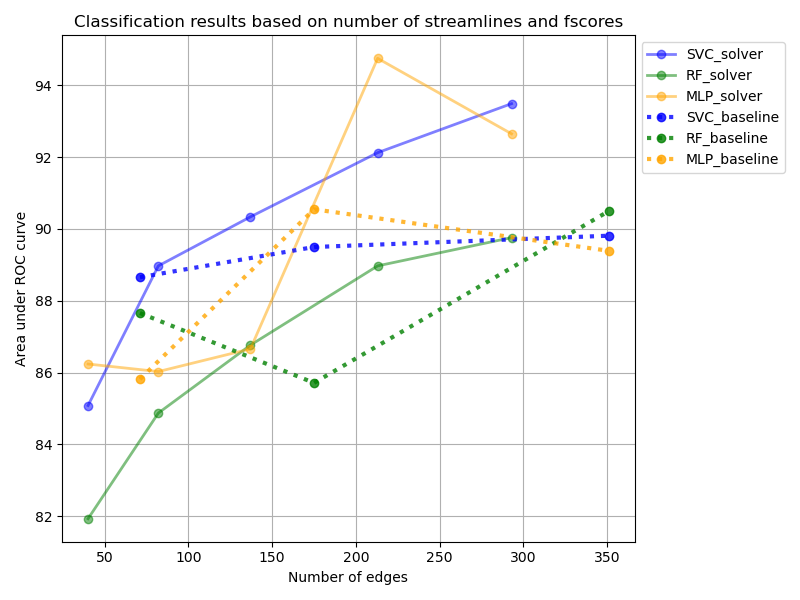
\includegraphics[height=0.5\textwidth, width=0.7\textwidth, keepaspectratio]{images/select_clf_auc_gender.png}
    \caption{Comparison of \gls{AUC} for gender classification on the independent test set. The performance of three classifiers \gls{SVC}, \gls{RF2} and \gls{MLP} on basis is compared. The solid lines and dashed lines represent the performance for features filtered according to the solver and baseline experiments respectively.}
    \label{fig:clf_solver results}
\end{figure}
\begin{figure}[]
    \centering
    %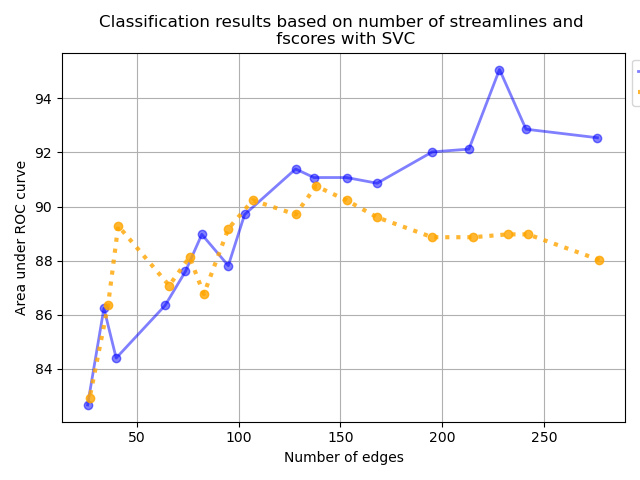
\includegraphics[width=0.8\textwidth]{images/select_clf_auc_gender_2_svc.png}
    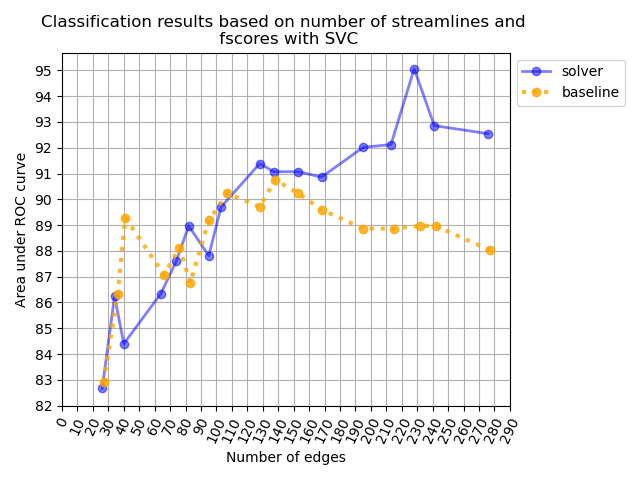
\includegraphics[height=0.5\textwidth, width=0.7\textwidth, keepaspectratio]{images/select_clf_auf_gender_2_scaled.png}
    \caption{Comparison of solver and baseline for gender classification with almost the same number of features selected in each case. The streamline count is used as the connectivity metric and f-scores are used as the feature scoring technique. }
    \label{fig:svcgender}
\end{figure}
\begin{figure}[]
    \centering
    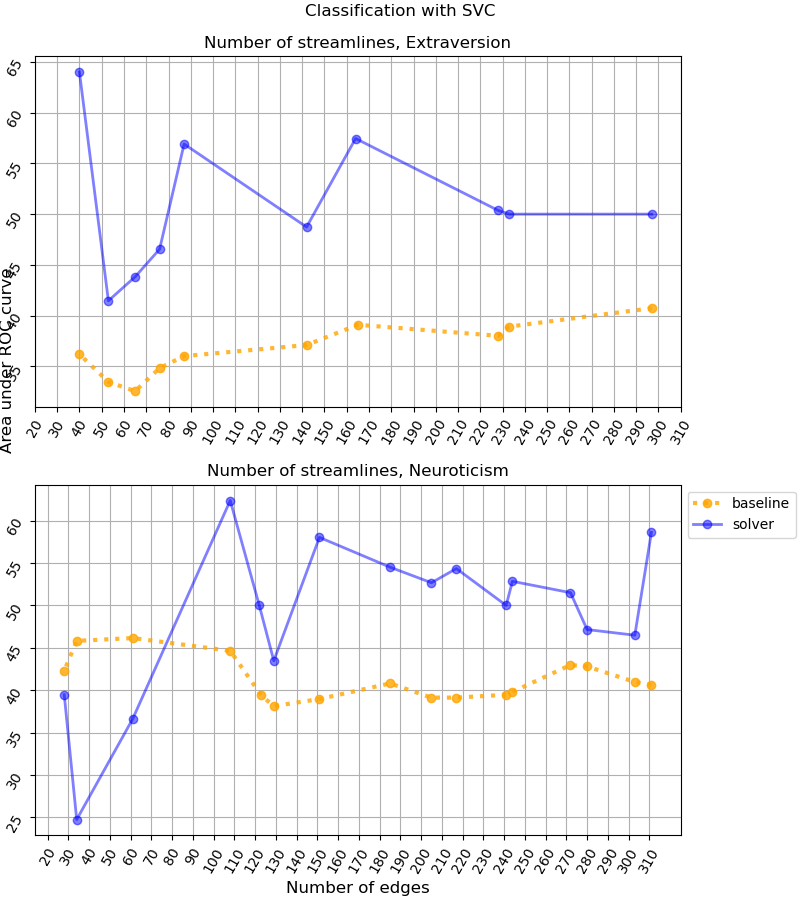
\includegraphics[width=\textwidth]{images/persona_comp.png}
    \caption{Comparison of solver and baseline for classification of personality traits using \gls{SVC}. This figure represents an exhaustive search carried out for only two out of five personality traits with the streamline count as the connectivity metric and Pearson correlation as the feature scoring technique. The cases represented in this figure have been selected due to the reasons mentioned in \autoref{res:baseline}.}
    \label{fig:persona_com}
\end{figure}
For the classification of gender, the comparison of classification performance was easily interpretable. At first, the baseline experiments for $k \in \{2,5,10\}$ were compared with solver nodes $m \in \{5,10,15,25,30\}$ due to computational complexity of the exhaustive search. \Cref{fig:clf_solver results} was used to determine the which classifier performs the best and gives results free from overfitting. 

The \gls{SVC} based classification produced the most stable results out of the three classifiers used and was taken as the choice for an exhaustive search. Once the classifier was decided upon, classification performance for a higher number of data points was determined.  This time the parameter top $k$ percentile of features to be preserved with the baseline was decided by using the polynomial in \cref{fig:fun_num_edges} so that the number of edges selected by the solver and the baseline are similar and classification results can be easily compared. 

The subsequent results using \gls{SVC} (\cref{fig:svcgender}) clearly indicate a cutoff number of edges, i.e. precisely 137 (obtained from the function in \cref{fig:fun_num_edges}). The \gls{MEWIS} solver does better than the baseline analysis in terms of classification performance after the cutoff value of 137 edges. Even for the number of edges below 137, the classification performance of both the methods remains comparable.  It can be inferred that preserving more than 137 edges or 20 nodes (according to \cref{fig:fun_num_edges}) with the \gls{MEWIS} offers more interpretability as well as better classification performance than the baseline method. This means that with $m> 20$ nodes, there is a decrease in interpretability but an increase in classifier performance. Preserving less than 20 nodes leads to a reduction in classifier performance but an increase in ease of visualization and interpretability.

The use cases in \cref{fig:persona base} was used to carry out an exhaustive search for the comparison of model performance between the two feature selection techniques. \cref{fig:persona_com} highlights this comparison. The \gls{MEWIS} method performed much better than baseline analysis throughout the range of feature numbers. For the classification of neuroticism the solver is able to achieve a maximum \gls{AUC} of around 64\% which is a better than the maximum score of 40\% by a margin of 24\%. Similarly, for neuroticism the \gls{SVC} achieves about 62\% accuracy with the \gls{MEWIS} solver and a little over 45\% for the baseline. One important detail to note is that the baseline performance might not exactly be the same as that in \cref{fig:persona base} since the number of features used for classification is not the same.

On the basis of the classification results for personality traits and gender, it can be concluded that the \gls{MEWIS} solver is a better feature selection technique than the baseline analysis.

%\subsection{Best parameters}

% Best estimator {'solver': 'adam', 'learning_rate': 'adaptive', 'hidden_layer_sizes': (50, 100, 100, 50), 'alpha': 0.05, 'activation': 'relu'}
% ('MLP', 'Gender', 'random', 'f-scores', 'baseline', 'num_streamlines', 5, 'balanced_accuracy', False)
%Bet estimator {'solver': 'adam', 'learning_rate': 'adaptive', 'hidden_layer_sizes': (50, 100, 100, 50), 'alpha': 0.05, 'activation': 'tanh'}
\begin{table}[t]
\begin{tcolorbox}
    \centering
    \begin{tabular}{!{\vrule width 2pt}c|c|c!{\vrule width 2pt}}
        \specialrule{0.2em}{0.01em}{0.01em}
        Hyperparameter & Solver & baseline \\
        \hline
        C & 5.9 & 0.522\\
        \hline
        Gamma &  4e-4 &  8e-4\\
        \hline
        kernel &  rbf & rbf\\
        \hline
        class weight & balanced & None\\
        \specialrule{0.2em}{0.01em}{0.01em}
    \end{tabular}
    \caption{Cross validation parameters for SVC trained for gender classification. The parameters which give the best area under the curve for the use case mentioned in the section above have been presented}
    \label{tab:CSV best parameters}
\end{tcolorbox}
\end{table}

In the remainder of this section, the parameters of the best estimators for gender classification will be presented. The \gls{SVC} gave most stable results as compared to other classifiers. The best performing estimators are determined using \cref{fig:svcgender}. For gender classification using the solver, the maximum \gls{AUC} of 95\% for the independent test set could be achieved. This performance is obtained for 237 edges corresponding to 26 nodes. Using the baseline technique, the best estimator could achieve 91\% area under curve  for around 138 edges.

In \autoref{tab:CSV best parameters} the parameters of the best estimators for the MEWIS solver based method and baseline used for gender classification using number of streamlines and f-scores will be presented.


%Best estimator {'C': 5.918565074193836, 'class_weight': 'balanced', 'gamma': 0.0004643818614121193, 'kernel': 'rbf'}
%Best estimator basline {'C': 0.5229762127721259, 'class_weight': None, 'gamma': 0.008523831363402392, 'kernel': 'rbf'}



\end{document}
